\documentclass{scrartcl}

\usepackage{geometry}
\geometry{
	paper=a4paper, % Paper size
	top=2cm, % Top margin
	bottom=2cm, % Bottom margin
	left=2cm, % Left margin
	right=2cm, % Right margin
	headheight=0.75cm, % Header height
	footskip=1.5cm, % Space from the bottom margin to the baseline of the footer
	headsep=0.75cm, % Space from the top margin to the baseline of the header
	%showframe, % Uncomment to show how the type block is set on the page
}

\usepackage{tabularx}
\usepackage{booktabs}
\usepackage{blindtext}
% Character encoding
\usepackage[T1]{fontenc}
\usepackage[utf8]{inputenc}
% Mathematics packages from AMS
\usepackage{amsmath, amsfonts, amsthm, amssymb}
\usepackage{braket, nicefrac}
% International System of Units
\usepackage{siunitx}
% Lists / numbers
\usepackage{enumitem, multicol}
% Figure insertions
% Use option [H] to force the placement of a figure
\usepackage{graphicx, float}
\usepackage{keystroke}
\usepackage{pgfplots}\usepgfplotslibrary{units}\pgfplotsset{compat=1.16}
% Depth of the ToC
\setcounter{tocdepth}{3}
% Hyperlink References
\usepackage{hyperref}
\usepackage{enumitem}

\setlist{resume,leftmargin=8mm,label=\arabic*.,itemsep=-0.5mm,topsep=-3mm}

% Storage Path for images
\graphicspath{{images/}}

\setkomafont{disposition}{\normalfont\bfseries}

% Environments
\renewenvironment{abstract}{
    \begin{center}
    {\Large \textbf{Abstract}}
    \vspace{0.5cm}
    \par\itshape
    \begin{minipage}{0.8\linewidth}}{\end{minipage}
    \noindent\ignorespaces
    \end{center}
}

\newenvironment{preface}{
  \begin{center}
    {\Large \textbf{Preface}}
    \vspace{0.5cm}
    \par
    \begin{minipage}{0.8\linewidth}}{\end{minipage}
    \noindent\ignorespaces
  \end{center}
}


\begin{document}
%Title of the report, name of coworkers and dates (of experiment and of report).
\begin{titlepage}
	\centering
	
\includegraphics[width=0.2\textwidth]{al-azhar.png}\par\vspace{12pt}
	{\LARGE Al-Azhar University \par}\vspace{3pt}
	{\Large Faculty of Engineering \par}
	{\Large Computers \& Systems Engineering Department \par}\vspace{12pt}
	\vfill
	{\huge\bfseries\scshape Web Page Ranking \par}\vspace{8pt}
  {\scshape Seo Suggestion Search Engine Project \par}\vspace{8pt}
  {\itshape (Software Design Report) \par}
	\vfill
	{\Large\texttt{Contributors:} \\[12pt]
    \Large\itshape\ttfamily
    \begin{tabular}{ll}
      55 & Abd El-Twab M. Fakhry \\
      56 & Abd El-Hameed Hassan \\
      57 & Abd El-Khalek Alashker \\
      58 & Abdurrahman Khalefa \\
      59 & Abdurrahman Gamal \\
      60 & Abdurrahman Ramadan \\
    \end{tabular}
  }\par
	\vspace{1cm}
	\vfill
  {\Large\texttt{Supervised by:} \\
	\texttt{Dr. Muhammad Atef} \par}
  \vfill
  {\large \today \par}
\end{titlepage}

\newpage

\begin{preface}
  The purpose of a preface is to persuade your readers that they should read the rest of your written work. Keep it short. Describe your background and credentials. Discuss what inspired the project described in this report. Explain who your target audience is, and tell the reader why this project is important to them.
\end{preface}\vspace{1cm}

\begin{abstract}
  A strong abstract sums up your work in very few sentences:
  (i) state the problem you are addressing;
  (ii) say why it’s an interesting problem, and which issues are hard to tackle;
  (iii) give your approach towards solving the problem;
  (iv) say why and how well your approach solves the problem.
\end{abstract}\vspace{1cm}

\newpage

\tableofcontents

\newpage

\section{Introduction}

Your introduction briefly explains the problem you address, and what you've achieved towards solving the problem. It's an edited and updated version of your context and objectives from your topic outline document.

\section{User Stories}

Our system has two main actors: Administrator and User.

\subsection{Administrator Login}

\begin{table}[H]
  \caption{User Story 1}
  \begin{tabular}{p{0.18\linewidth} | p{0.72\linewidth}}
    \toprule
    User Story ID & US1
    \\\midrule
    Name & Administrator login
    \\\hline
    Statement & As an administrator, I want to login into the system, So that I can enter the admin area.
    \\\hline
    Priority & HIGH
    \\\hline
    Estimation & 3 pts
    \\\hline
    Direct actors & Administrator
    \\\hline
    Pre-Conditions & {
                     \begin{enumerate}
                     \item Has internet access.
                     \item Has a browser.
                     \item Opens the login page in the browser.
                     \end{enumerate}
                     }\vspace*{-\baselineskip}
    \\\hline
    Post-Conditions & {
                      \begin{enumerate}
                      \item Feeds the database website URLs and their metadata.
                      \item Views the page ranking.
                      \end{enumerate}
                      }\vspace*{-\baselineskip}
    \\\hline
    Senario & {
              \begin{enumerate}
              \item The administrator fills in username and password fields.
              \item The administrator clicks on the admin login button.
              \item The system will validate the username and password. If correct, log in; otherwise, stay on the current login page.
              \item The system logs both correct and wrong login.
              \end{enumerate}
              }\vspace*{-\baselineskip}
    \\\bottomrule
  \end{tabular}
\end{table}

\subsection{Website URLs}

\begin{table}[H]
  \caption{User Story 2}
  \begin{tabular}{p{0.18\linewidth} | p{0.72\linewidth}}
    \toprule
    User Story ID & US2
    \\\midrule
    Name & Website URLs
    \\\hline
    Statement & As an administrator, I want to feed the database website URLs and their metadata, So that the system can use them to search the user query.
    \\\hline
    Priority & HIGH
    \\\hline
    Direct actors & Administrator
    \\\hline
    Pre-Conditions & {
                     \begin{enumerate}
                     \item US1.
                     \item Opens the Feed URLs page.
                     \end{enumerate}
                     }\vspace*{-\baselineskip}
    \\\hline
    Post-Conditions & -
    \\\hline
    Senario & {
              \begin{enumerate}
              \item The administrator feeds the database website URLs and its metadata.
              \item The administrator clicks on add new website button.
              \item The system saves the data in a new row in the database.
              \end{enumerate}
              }\vspace*{-\baselineskip}
    \\\bottomrule
  \end{tabular}
\end{table}

\subsection{Page Ranking}

\begin{table}[H]
  \caption{User Story 3}
  \begin{tabular}{p{0.18\linewidth} | p{0.72\linewidth}}
    \toprule
    User Story ID & US3
    \\\midrule
    Name & Page Ranking
    \\\hline
    Statement & As an administrator, I want to view the page rank, So that I can optimize the search functionality.
    \\\hline
    Priority & REGULAR
    \\\hline
    Direct actors & Administrator
    \\\hline
    Pre-Conditions & {
                     \begin{enumerate}
                     \item US1.
                     \item Opens the Page Ranking page.
                     \end{enumerate}
                     }\vspace*{-\baselineskip}
    \\\hline
    Post-Conditions & -
    \\\hline
    Senario & {
              \begin{enumerate}
              \item The administrator clicks the page ranking anchor in the tab menu.
              \item The system lists the website URLs in the database sorted based on their number of visits and points.
              \end{enumerate}
              }\vspace*{-\baselineskip}
    \\\bottomrule
  \end{tabular}
\end{table}

\subsection{User Login}

\begin{table}[H]
  \caption{User Story 4}
  \begin{tabular}{p{0.18\linewidth} | p{0.72\linewidth}}
    \toprule
    User Story ID & US4
    \\\midrule
    Name & User login
    \\\hline
    Statement & As a user, I want to login into the system, So that I can search for specific topics.
    \\\hline
    Priority & HIGH
    \\\hline
    Direct actors & User
    \\\hline
    Pre-Conditions & {
                     \begin{enumerate}
                     \item Has internet access.
                     \item Has a browser.
                     \item Opens the login page in the browser.
                     \end{enumerate}
                     }\vspace*{-\baselineskip}
    \\\hline
    Post-Conditions & {
                      \begin{enumerate}
                      \item Searches for a specific topic.
                      \item Searches for website keywords and meta-description.
                      \end{enumerate}
                      }\vspace*{-\baselineskip}
    \\\hline
    % Main Success Section = Use-Cases >> Diagrams
    Senario & {
              \begin{enumerate}
              \item The user fills in username and password fields.
              \item The user clicks on the login button.
              \item The system will validate the username and password. If correct, log in; otherwise, stay on the current login page.
              \item The system logs both correct and wrong login.
              \end{enumerate}
              }\vspace*{-\baselineskip}
    \\\bottomrule
  \end{tabular}
\end{table}

\subsection{Search Page}

\begin{table}[H]
  \caption{User Story 5}
  \begin{tabular}{p{0.18\linewidth} | p{0.72\linewidth}}
    \toprule
    User Story ID & US5
    \\\midrule
    Name & Search Page
    \\\hline
    Statement & As a user, I want to open the search page, So that I can use the search box.
    \\\hline
    Priority & HIGH
    \\\hline
    Direct actors & User
    \\\hline
    Pre-Conditions & {
                     \begin{enumerate}
                     \item US4.
                     \item Opens the search page page.
                     \end{enumerate}
                     }\vspace*{-\baselineskip}
    \\\hline
    Post-Conditions & {
                      \begin{enumerate}
                      \item Searches for a specific topic.
                      \end{enumerate}
                      }\vspace*{-\baselineskip}
    \\\hline
    Senario & {
              \begin{enumerate}
              \item The user clicks the search page anchor in the tab menu.
              \item The system opens the page of the search.
              \end{enumerate}
              }\vspace*{-\baselineskip}
    \\\bottomrule
  \end{tabular}
\end{table}

\subsection{Search Box}

\begin{table}[H]
  \caption{User Story 6}
  \begin{tabular}{p{0.18\linewidth} | p{0.72\linewidth}}
    \toprule
    User Story ID & US6
    \\\midrule
    Name & Search Box
    \\\hline
    Statement & As a user, I want a search box, So that I can write down my search query.
    \\\hline
    Priority & HIGH
    \\\hline
    Direct actors & User
    \\\hline
    Pre-Conditions & {
                     \begin{enumerate}
                     \item US4.
                     \item Opens the search page page.
                     \end{enumerate}
                     }\vspace*{-\baselineskip}
    \\\hline
    Post-Conditions & {
                      \begin{enumerate}
                      \item Clicks on URLs.
                      \end{enumerate}
                      }\vspace*{-\baselineskip}
    \\\hline
    % Main Success Section = Use-Cases >> Diagrams
    Senario & {
              \begin{enumerate}
              \item The user write down his/her search query in the search box.
              \item The user clicks the search button.
              \item The system uses this query and matches it with the content provided in URLs fed in the database.
              \item The system generates a list of related URLs.
              \item The user can then click on any URL in the generated list, and the URL will open the corresponding website.
              \item The system increases the number of visits to that URL in the database.
              \item The system goes to the web page URL to fetch its metadata and gives points according to page errors.
              \item The system updates the page's rank in the database according to the points the page gains and the number of visits.
              \end{enumerate}
              }\vspace*{-\baselineskip}
    \\\bottomrule
  \end{tabular}
\end{table}

\subsection{SEO Suggestions}

\begin{table}[H]
  \caption{User Story 7}
  \begin{tabular}{p{0.18\linewidth} | p{0.72\linewidth}}
    \toprule
    User Story ID & US7
    \\\midrule
    Name & SEO Suggestions
    \\\hline
    Statement & As a user, I want to search a live URL, So that I can get suitable keywords and meta descriptions.
    \\\hline
    Priority & HIGH
    \\\hline
    Direct actors & User
    \\\hline
    Pre-Conditions & {
                     \begin{enumerate}
                     \item US4.
                     \item Opens the SEO Suggestions page.
                     \end{enumerate}
                     }\vspace*{-\baselineskip}
    \\\hline
    Post-Conditions & -
    \\\hline
    Senario & {
              \begin{enumerate}
              \item The user write down a live URL in the search box.
              \item The user clicks the find keywords and meta-description button.
              \item The system goes and scans the web page URL, extracts its meta-features.
              \item The system then lists out suitable keywords related to the contents of the web page URL and a meta-description.
              \end{enumerate}
              }\vspace*{-\baselineskip}
    \\\bottomrule
  \end{tabular}
\end{table}

\section{Use-cases}

\subsection{Actors}

\subsubsection{Administrator}

\subsubsection{User}

\section{ERD Diagram}

\section{Testing Script}

\section{Conclusion}

\newpage

\bibliographystyle{IEEEtran}
\bibliography{references}

% \newpage

% To create Appendix with additional stuff
% Put data files, CAD drawings, additional sketches, etc.

\appendix
\section{Appendix}

\subsection{UI/UX Design}

\begin{figure}[H]
  \centering
  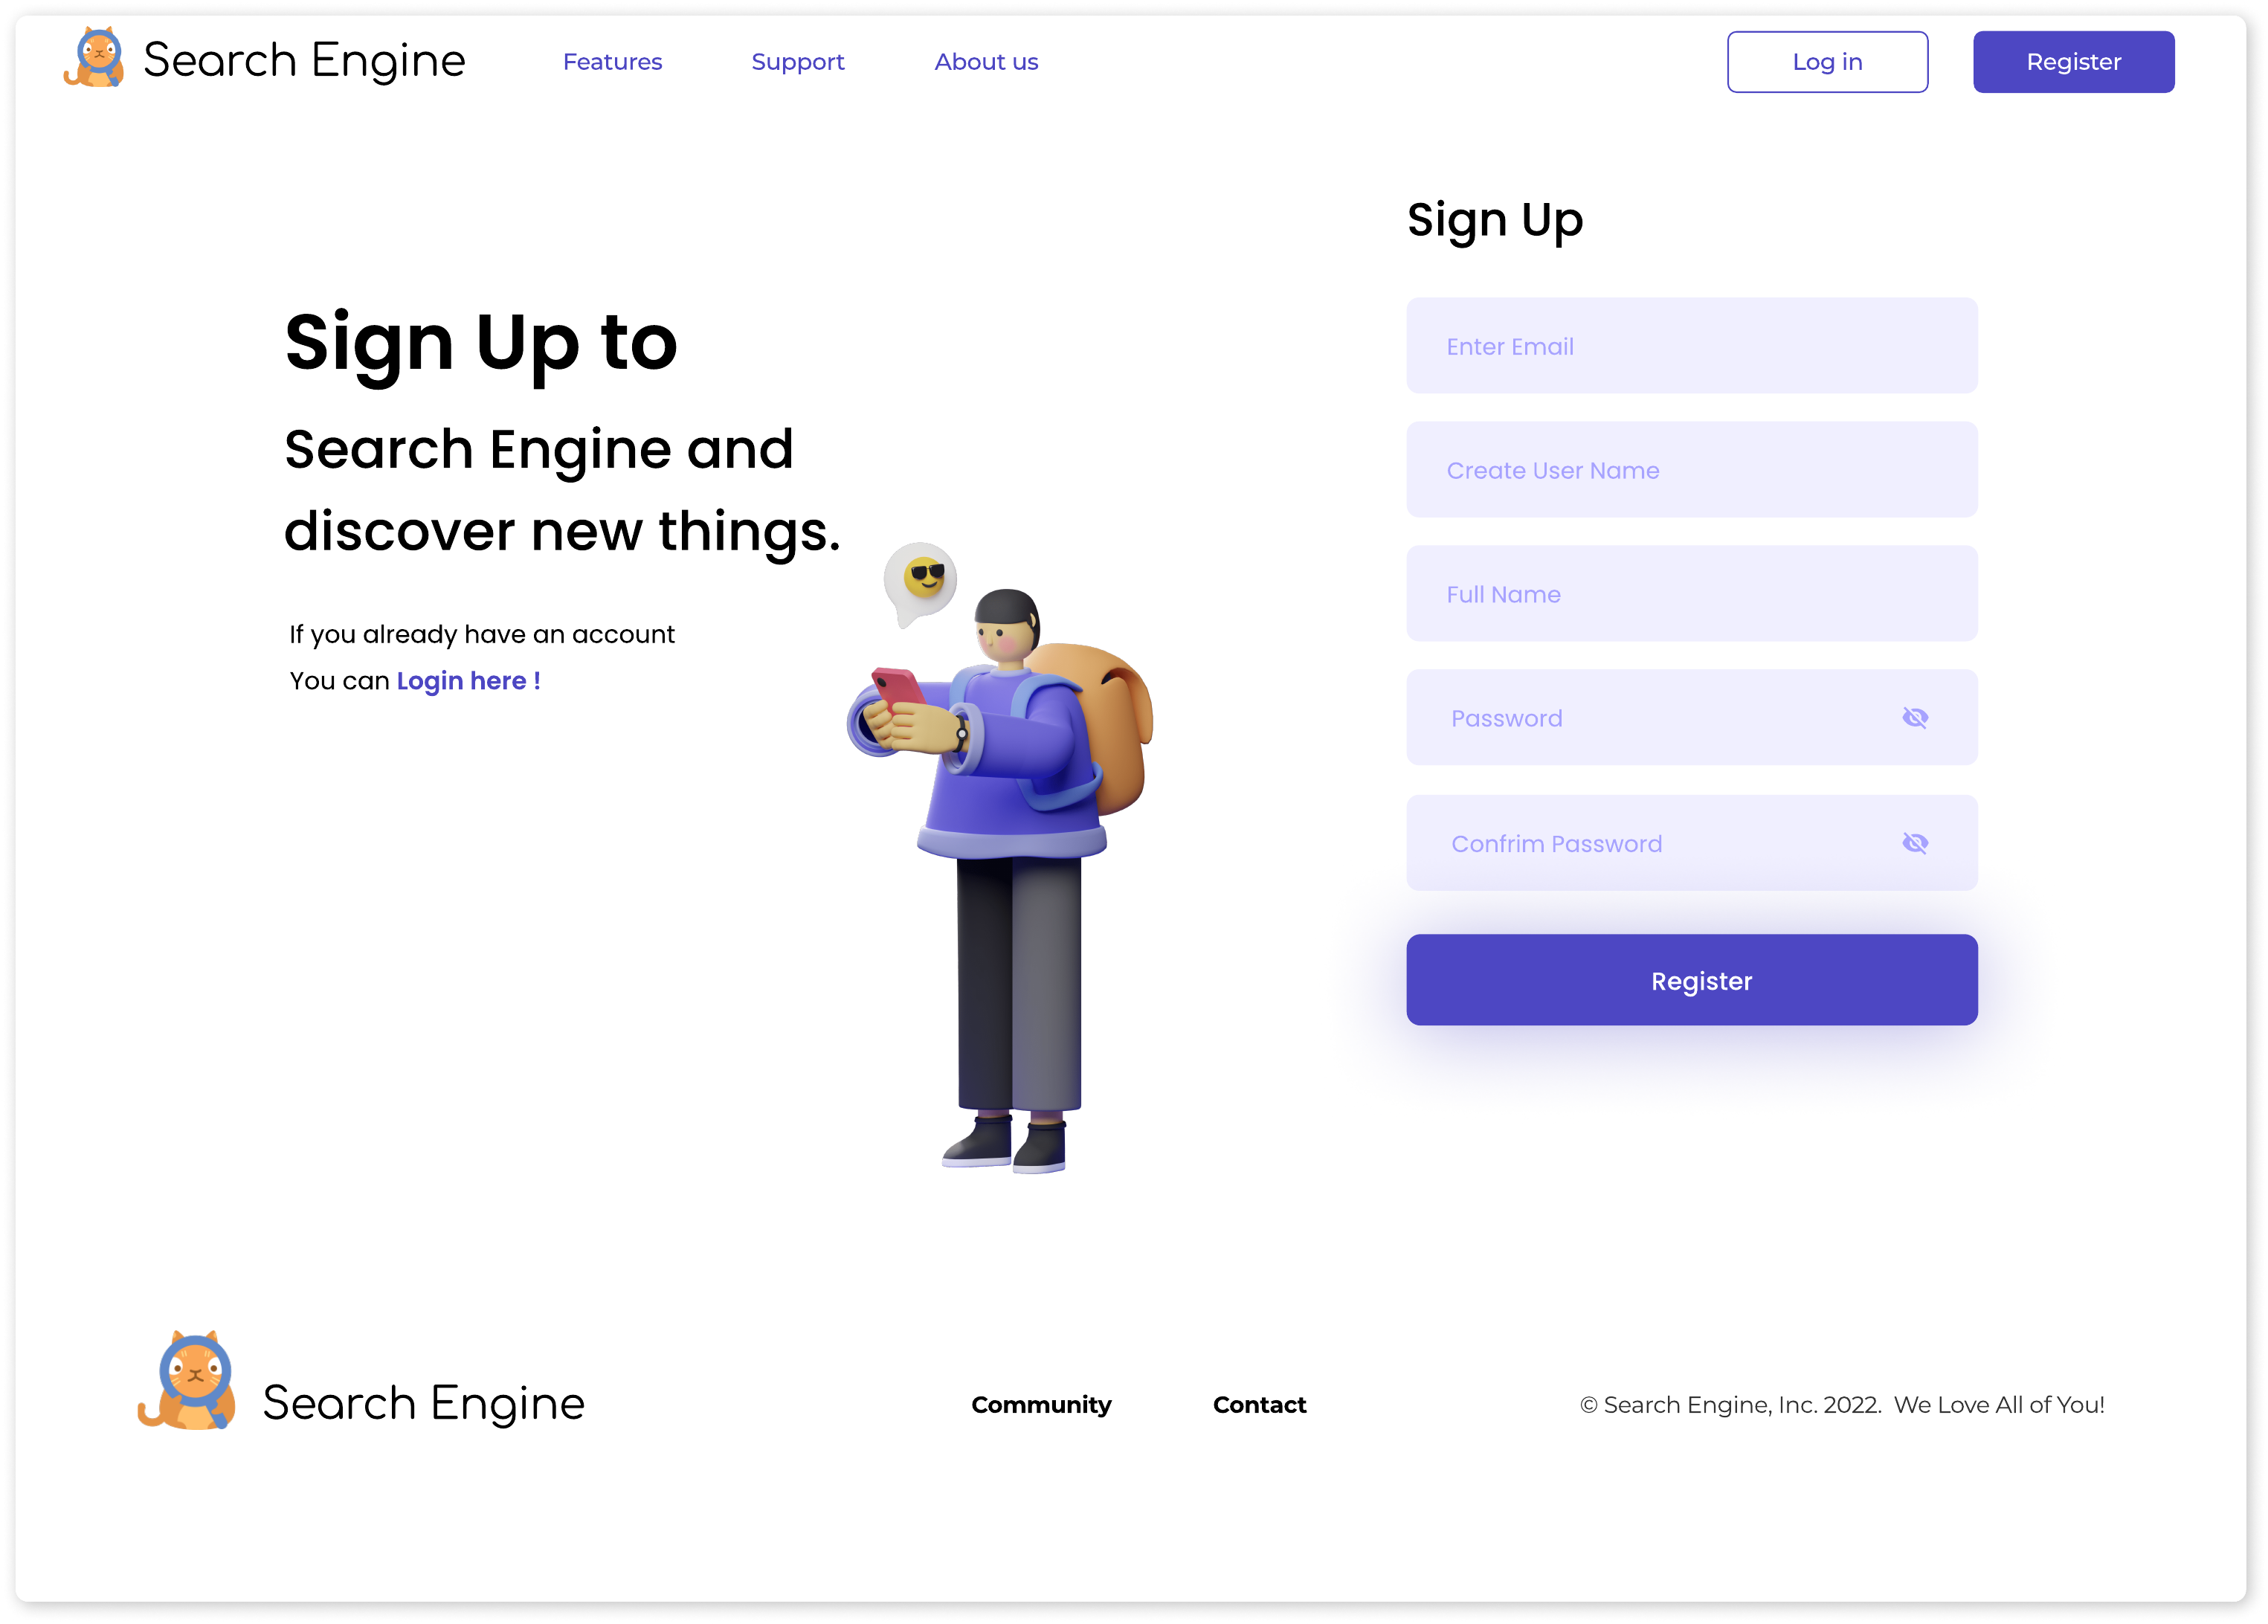
\includegraphics[width=0.90\textwidth]{register.pdf}
  \caption{Register Page}
\end{figure}

\begin{figure}[H]
  \centering
  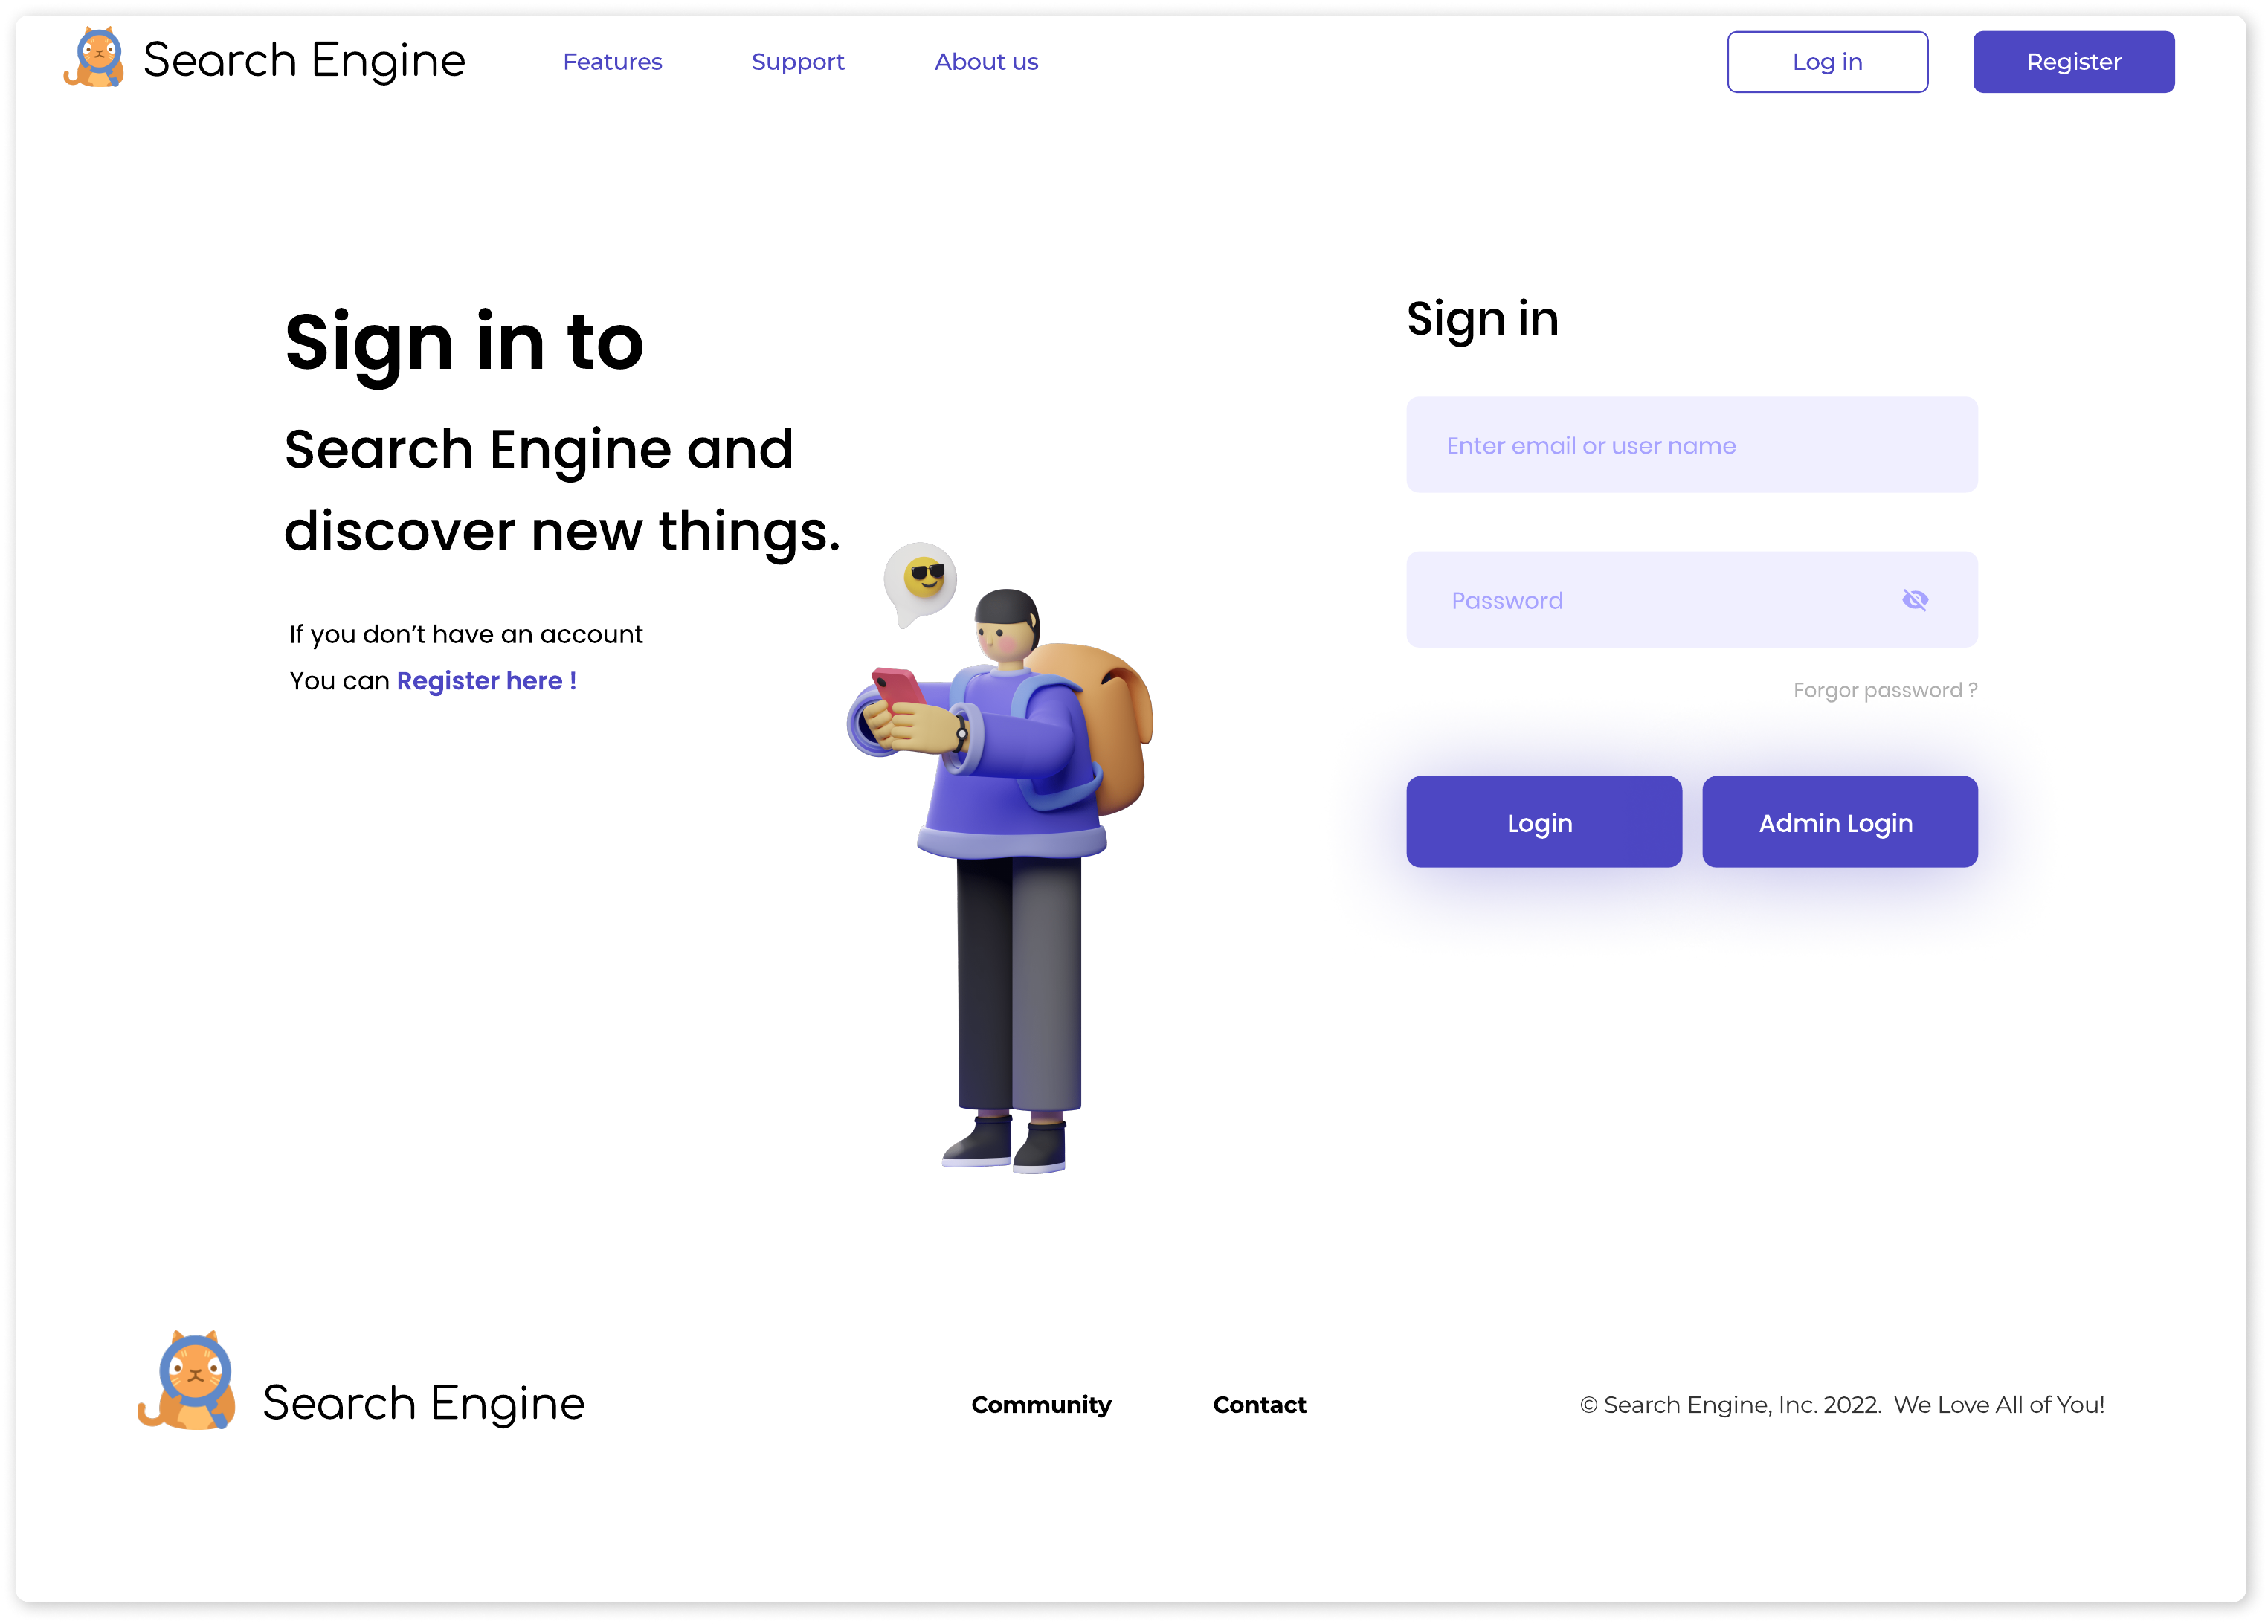
\includegraphics[width=0.90\textwidth]{login.pdf}
  \caption{Login Page}
\end{figure}

\begin{figure}[H]
  \centering
  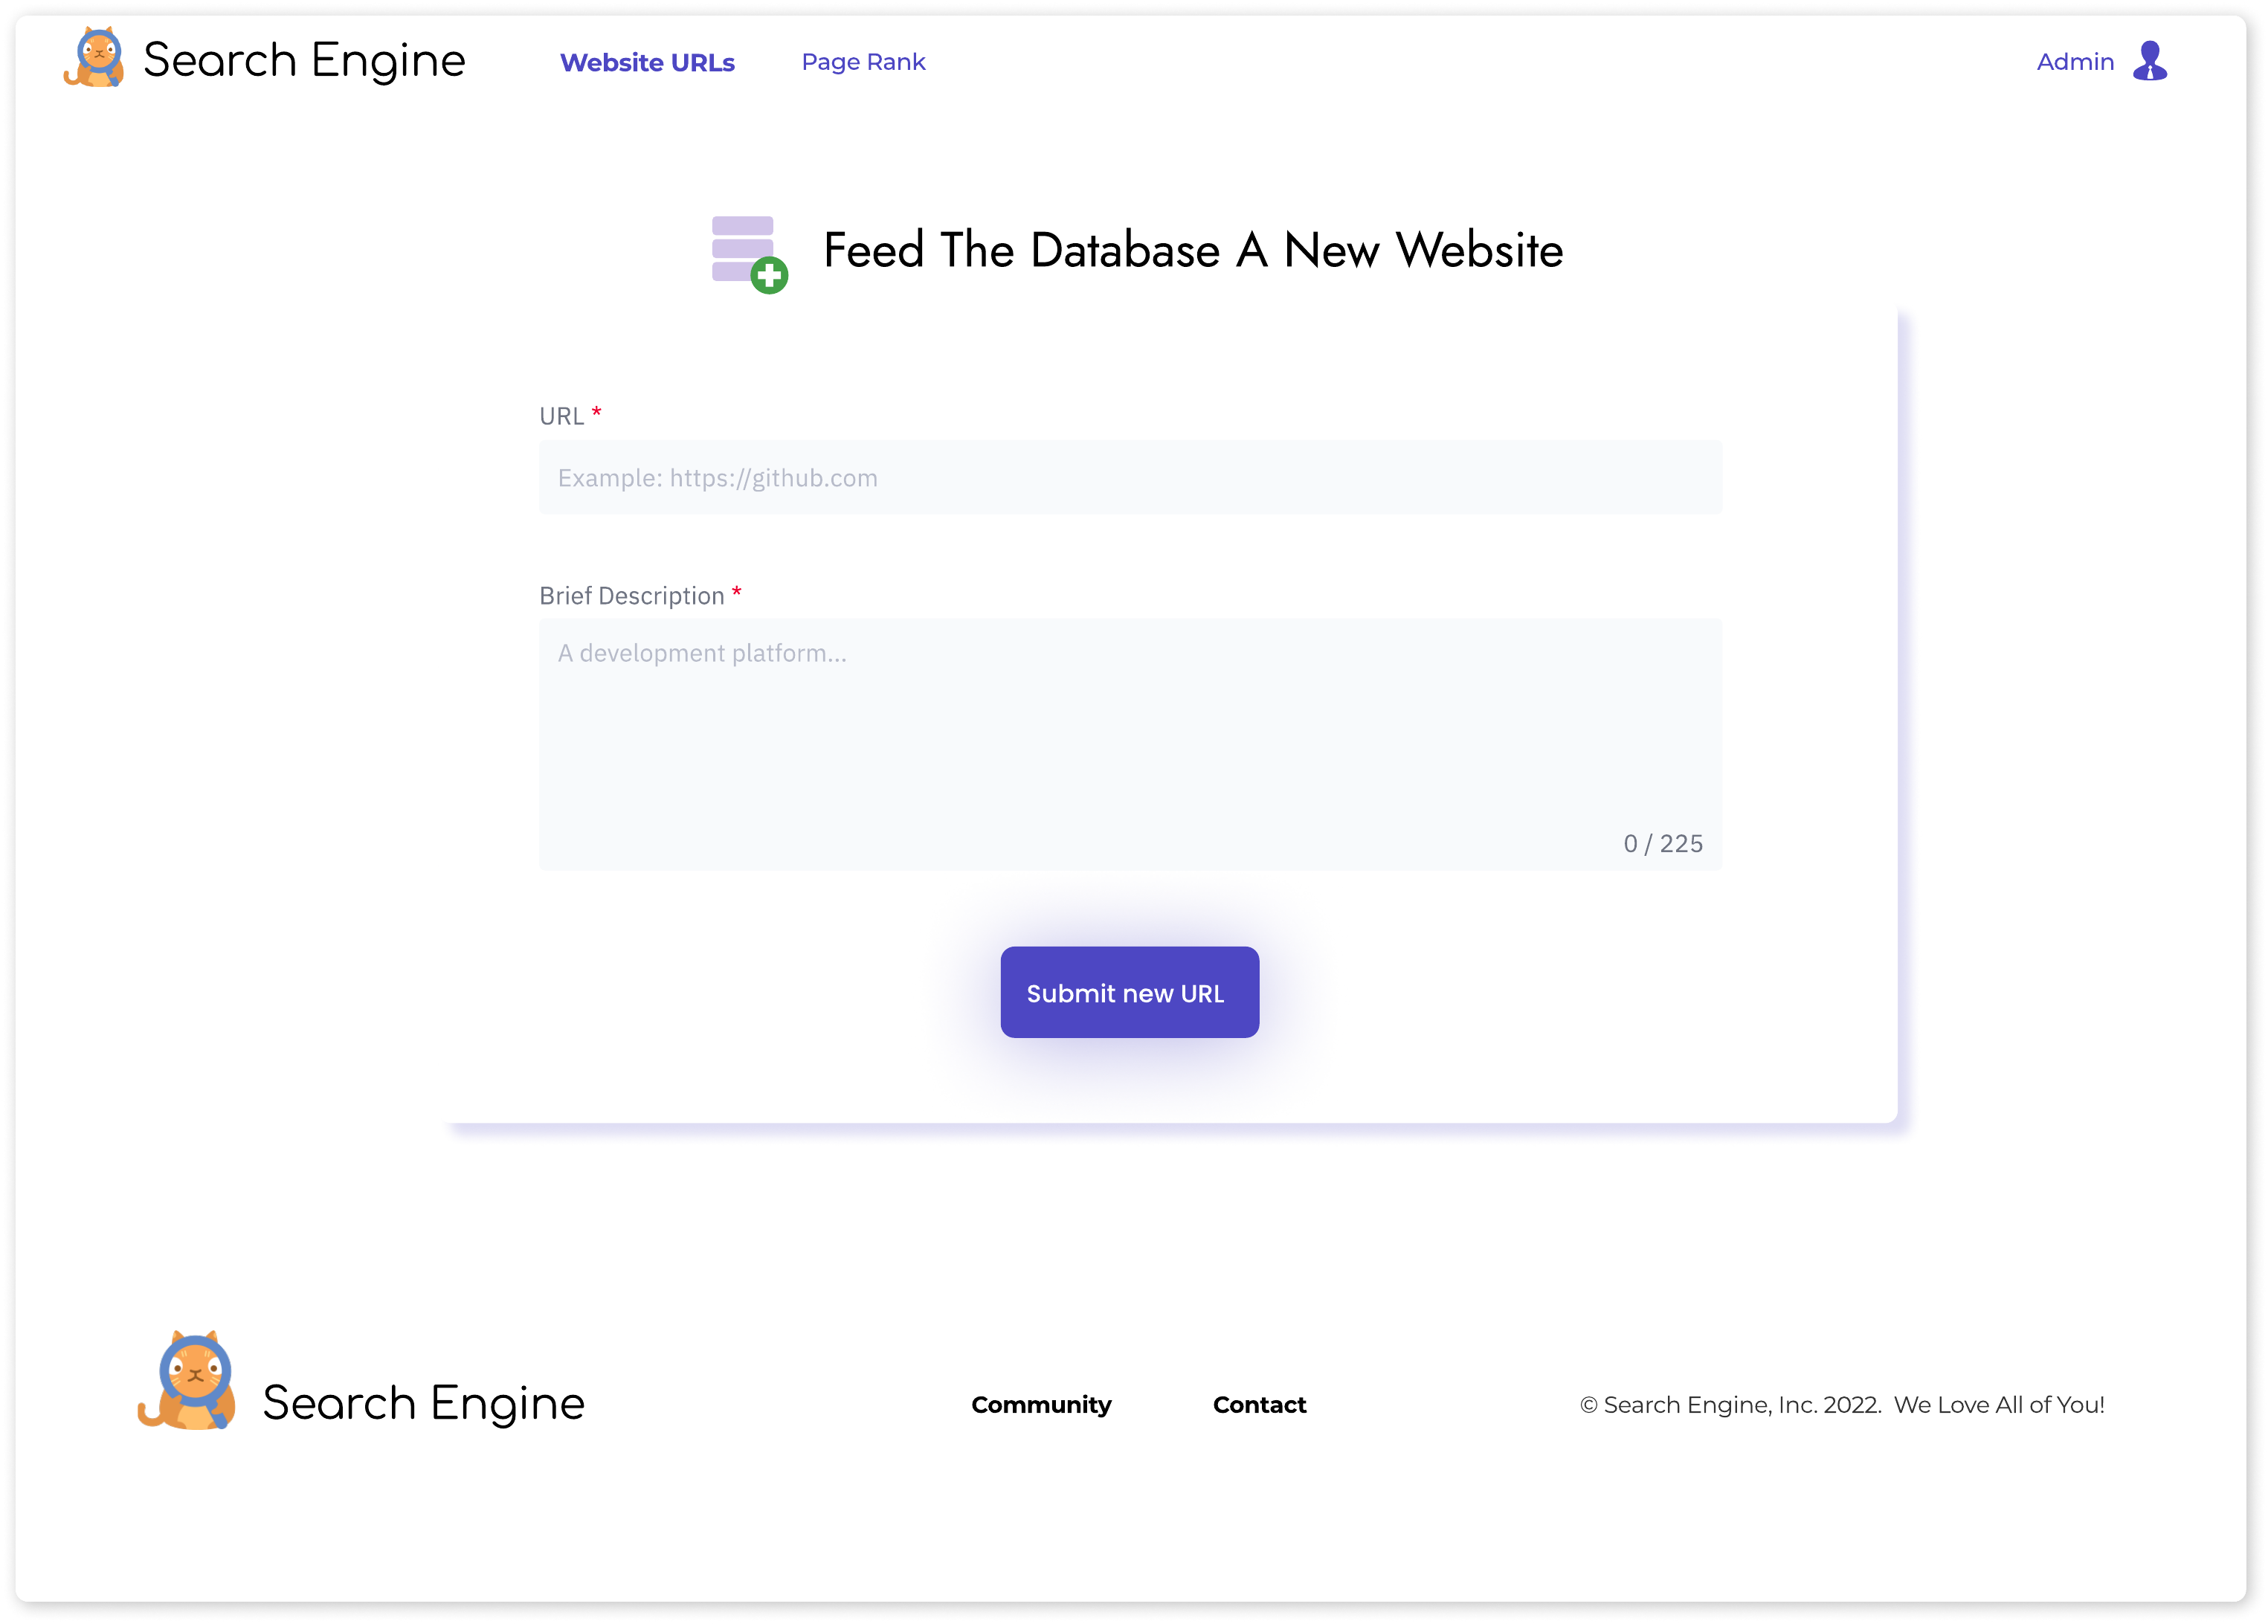
\includegraphics[width=0.90\textwidth]{website-urls.pdf}
  \caption{Website URLs}
\end{figure}

\begin{figure}[H]
  \centering
  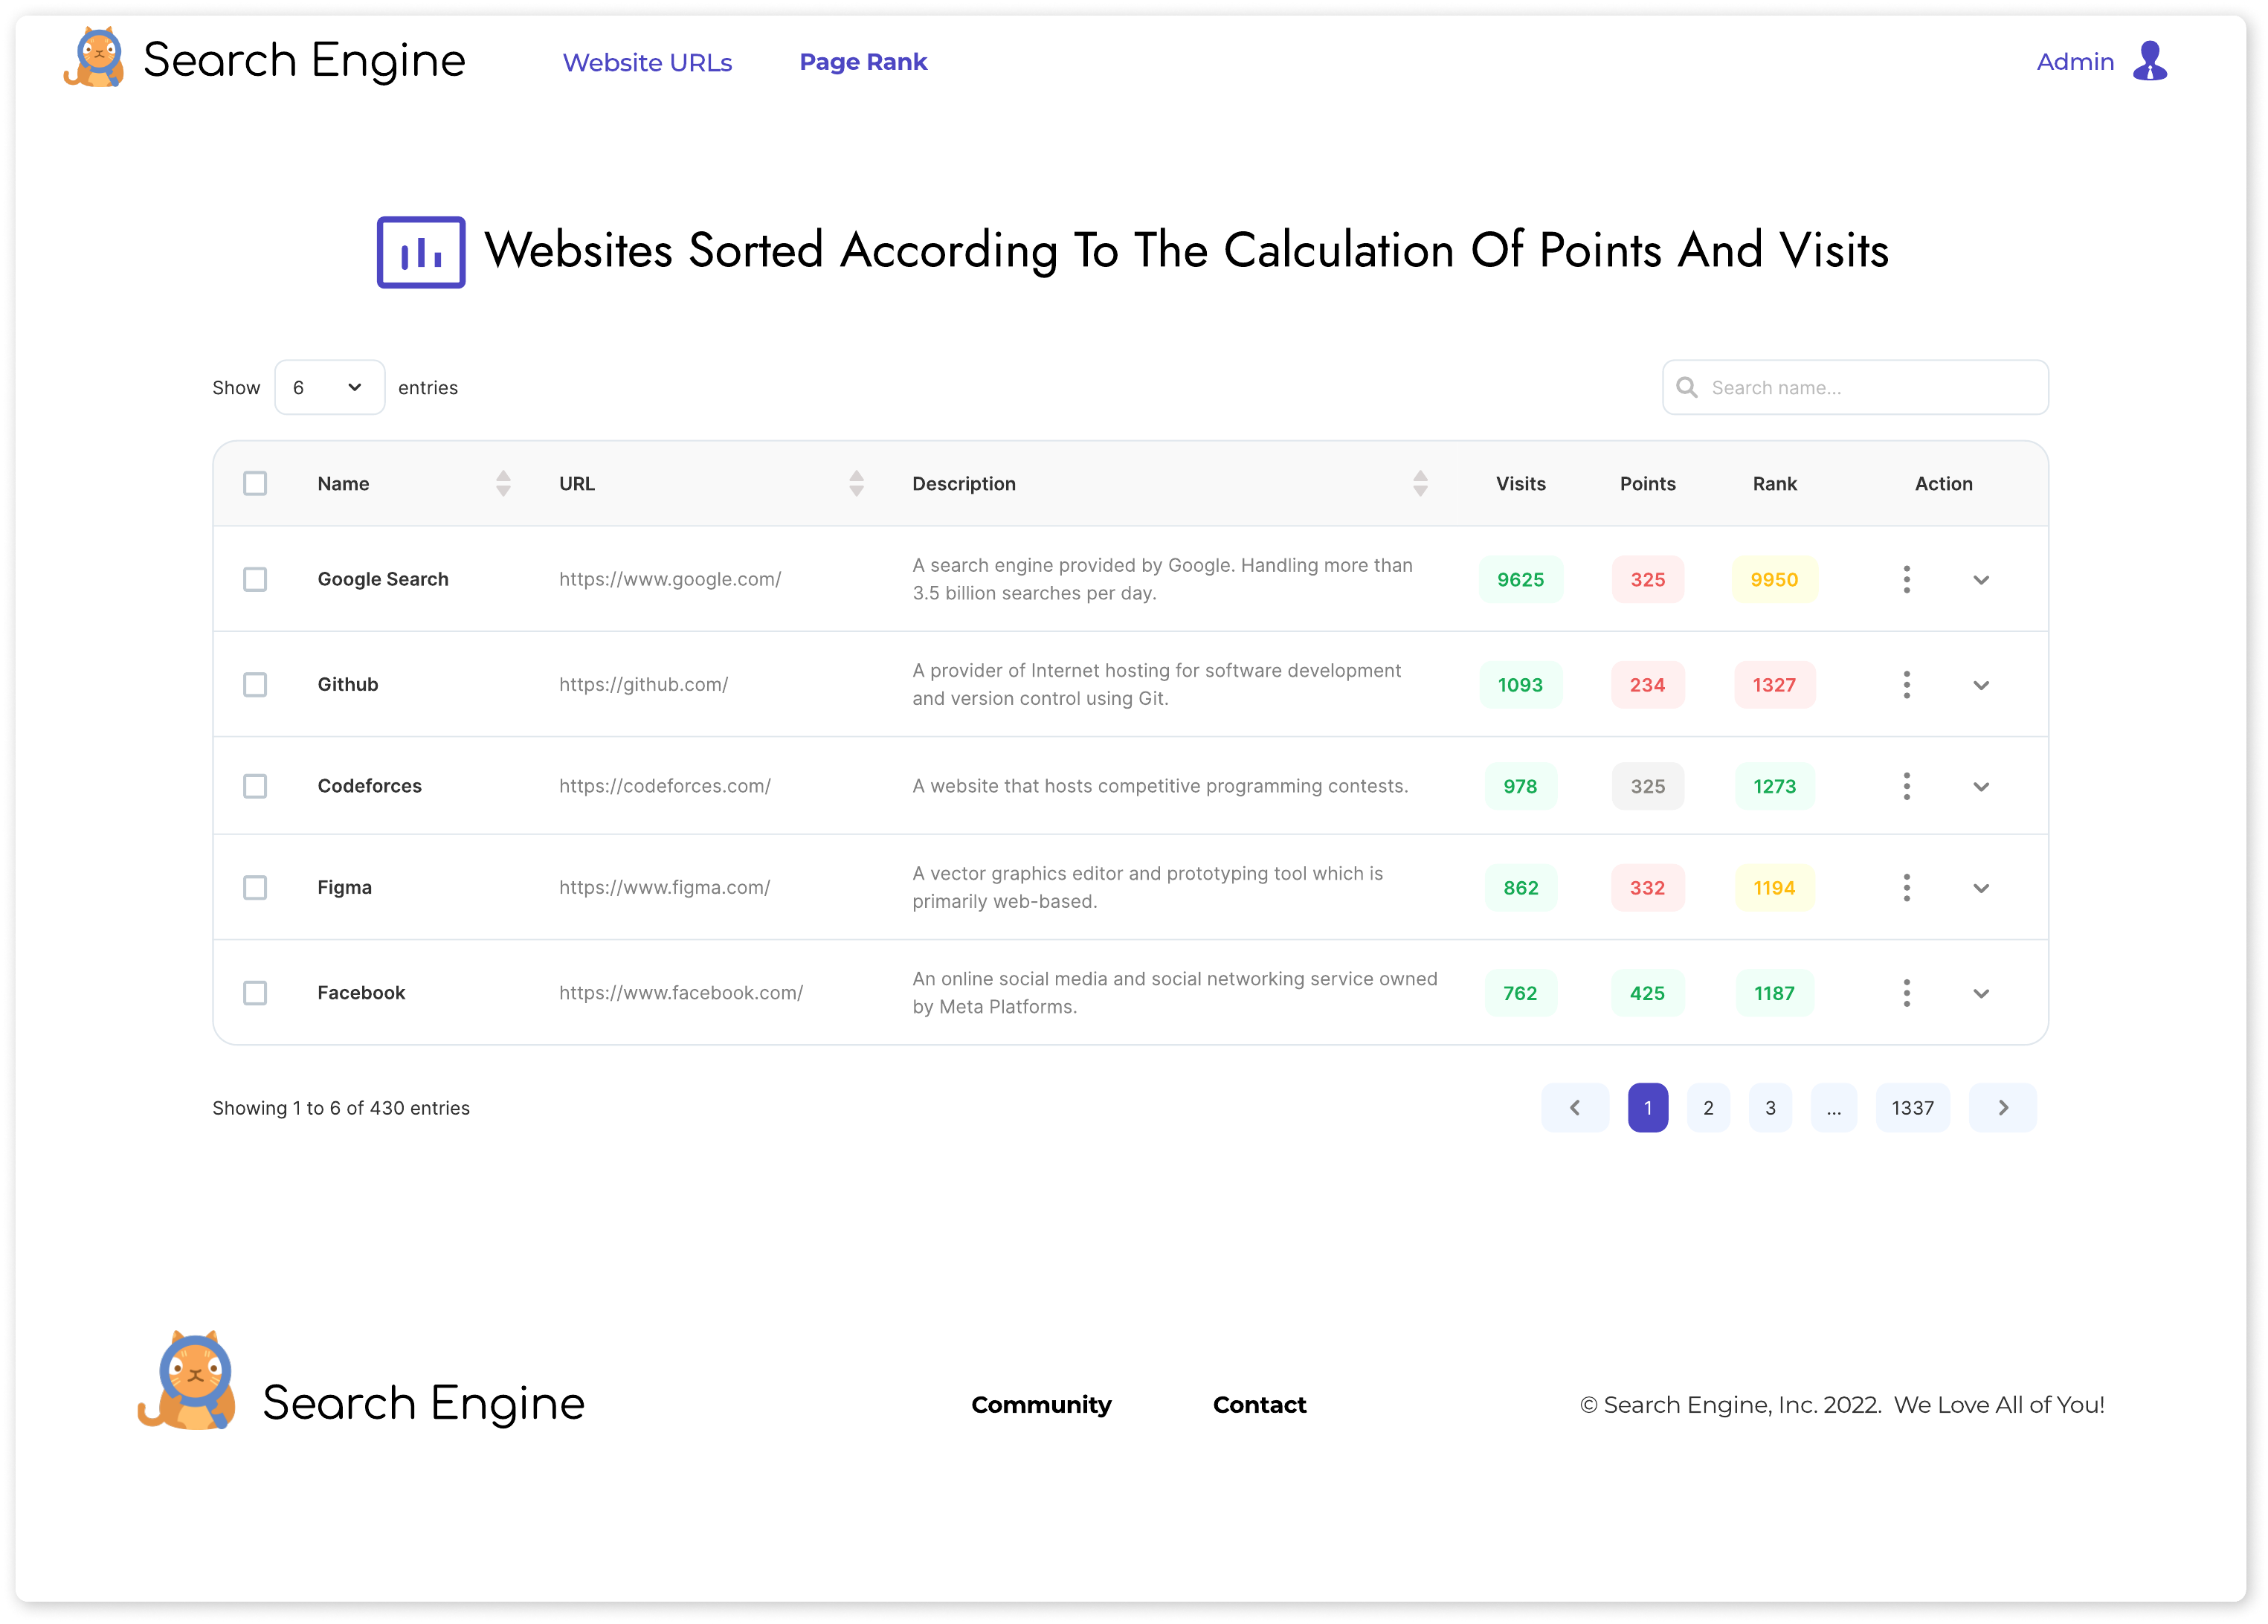
\includegraphics[width=0.90\textwidth]{page-rank.pdf}
  \caption{Page Rank}
\end{figure}

\begin{figure}[H]
  \centering
  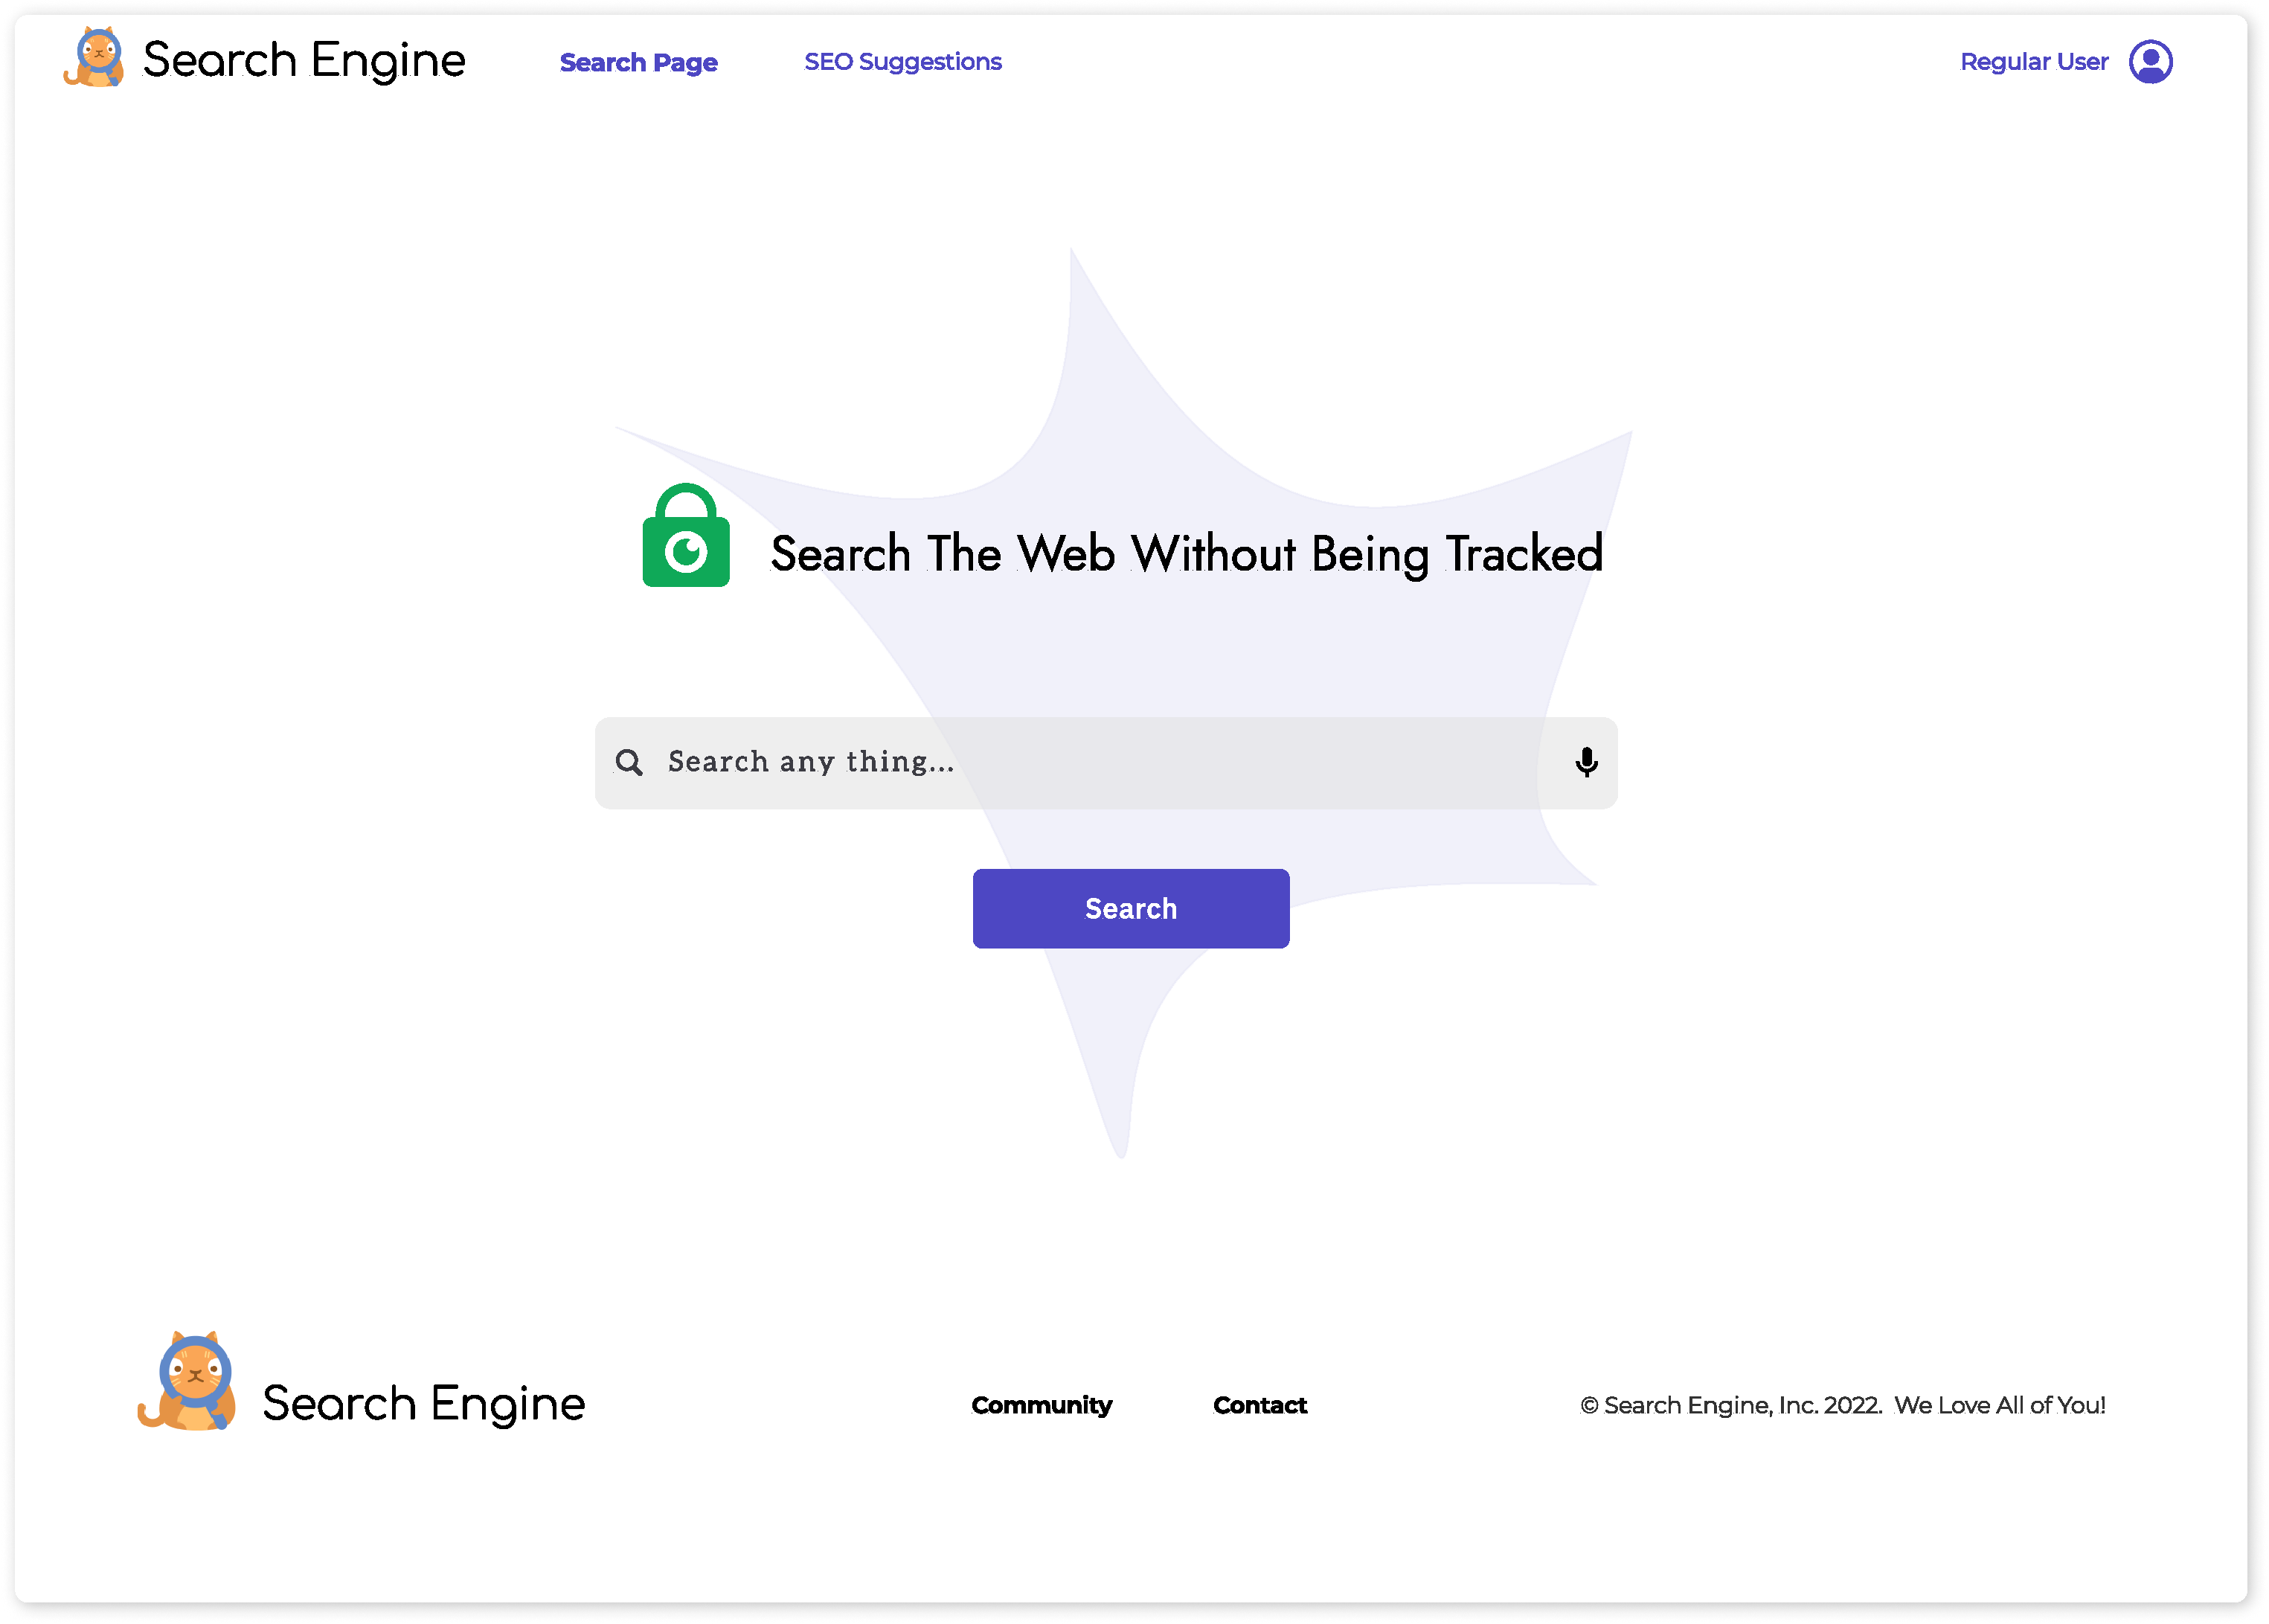
\includegraphics[width=0.90\textwidth]{search-box.pdf}
  \caption{Search Box}
\end{figure}

\begin{figure}[H]
  \centering
  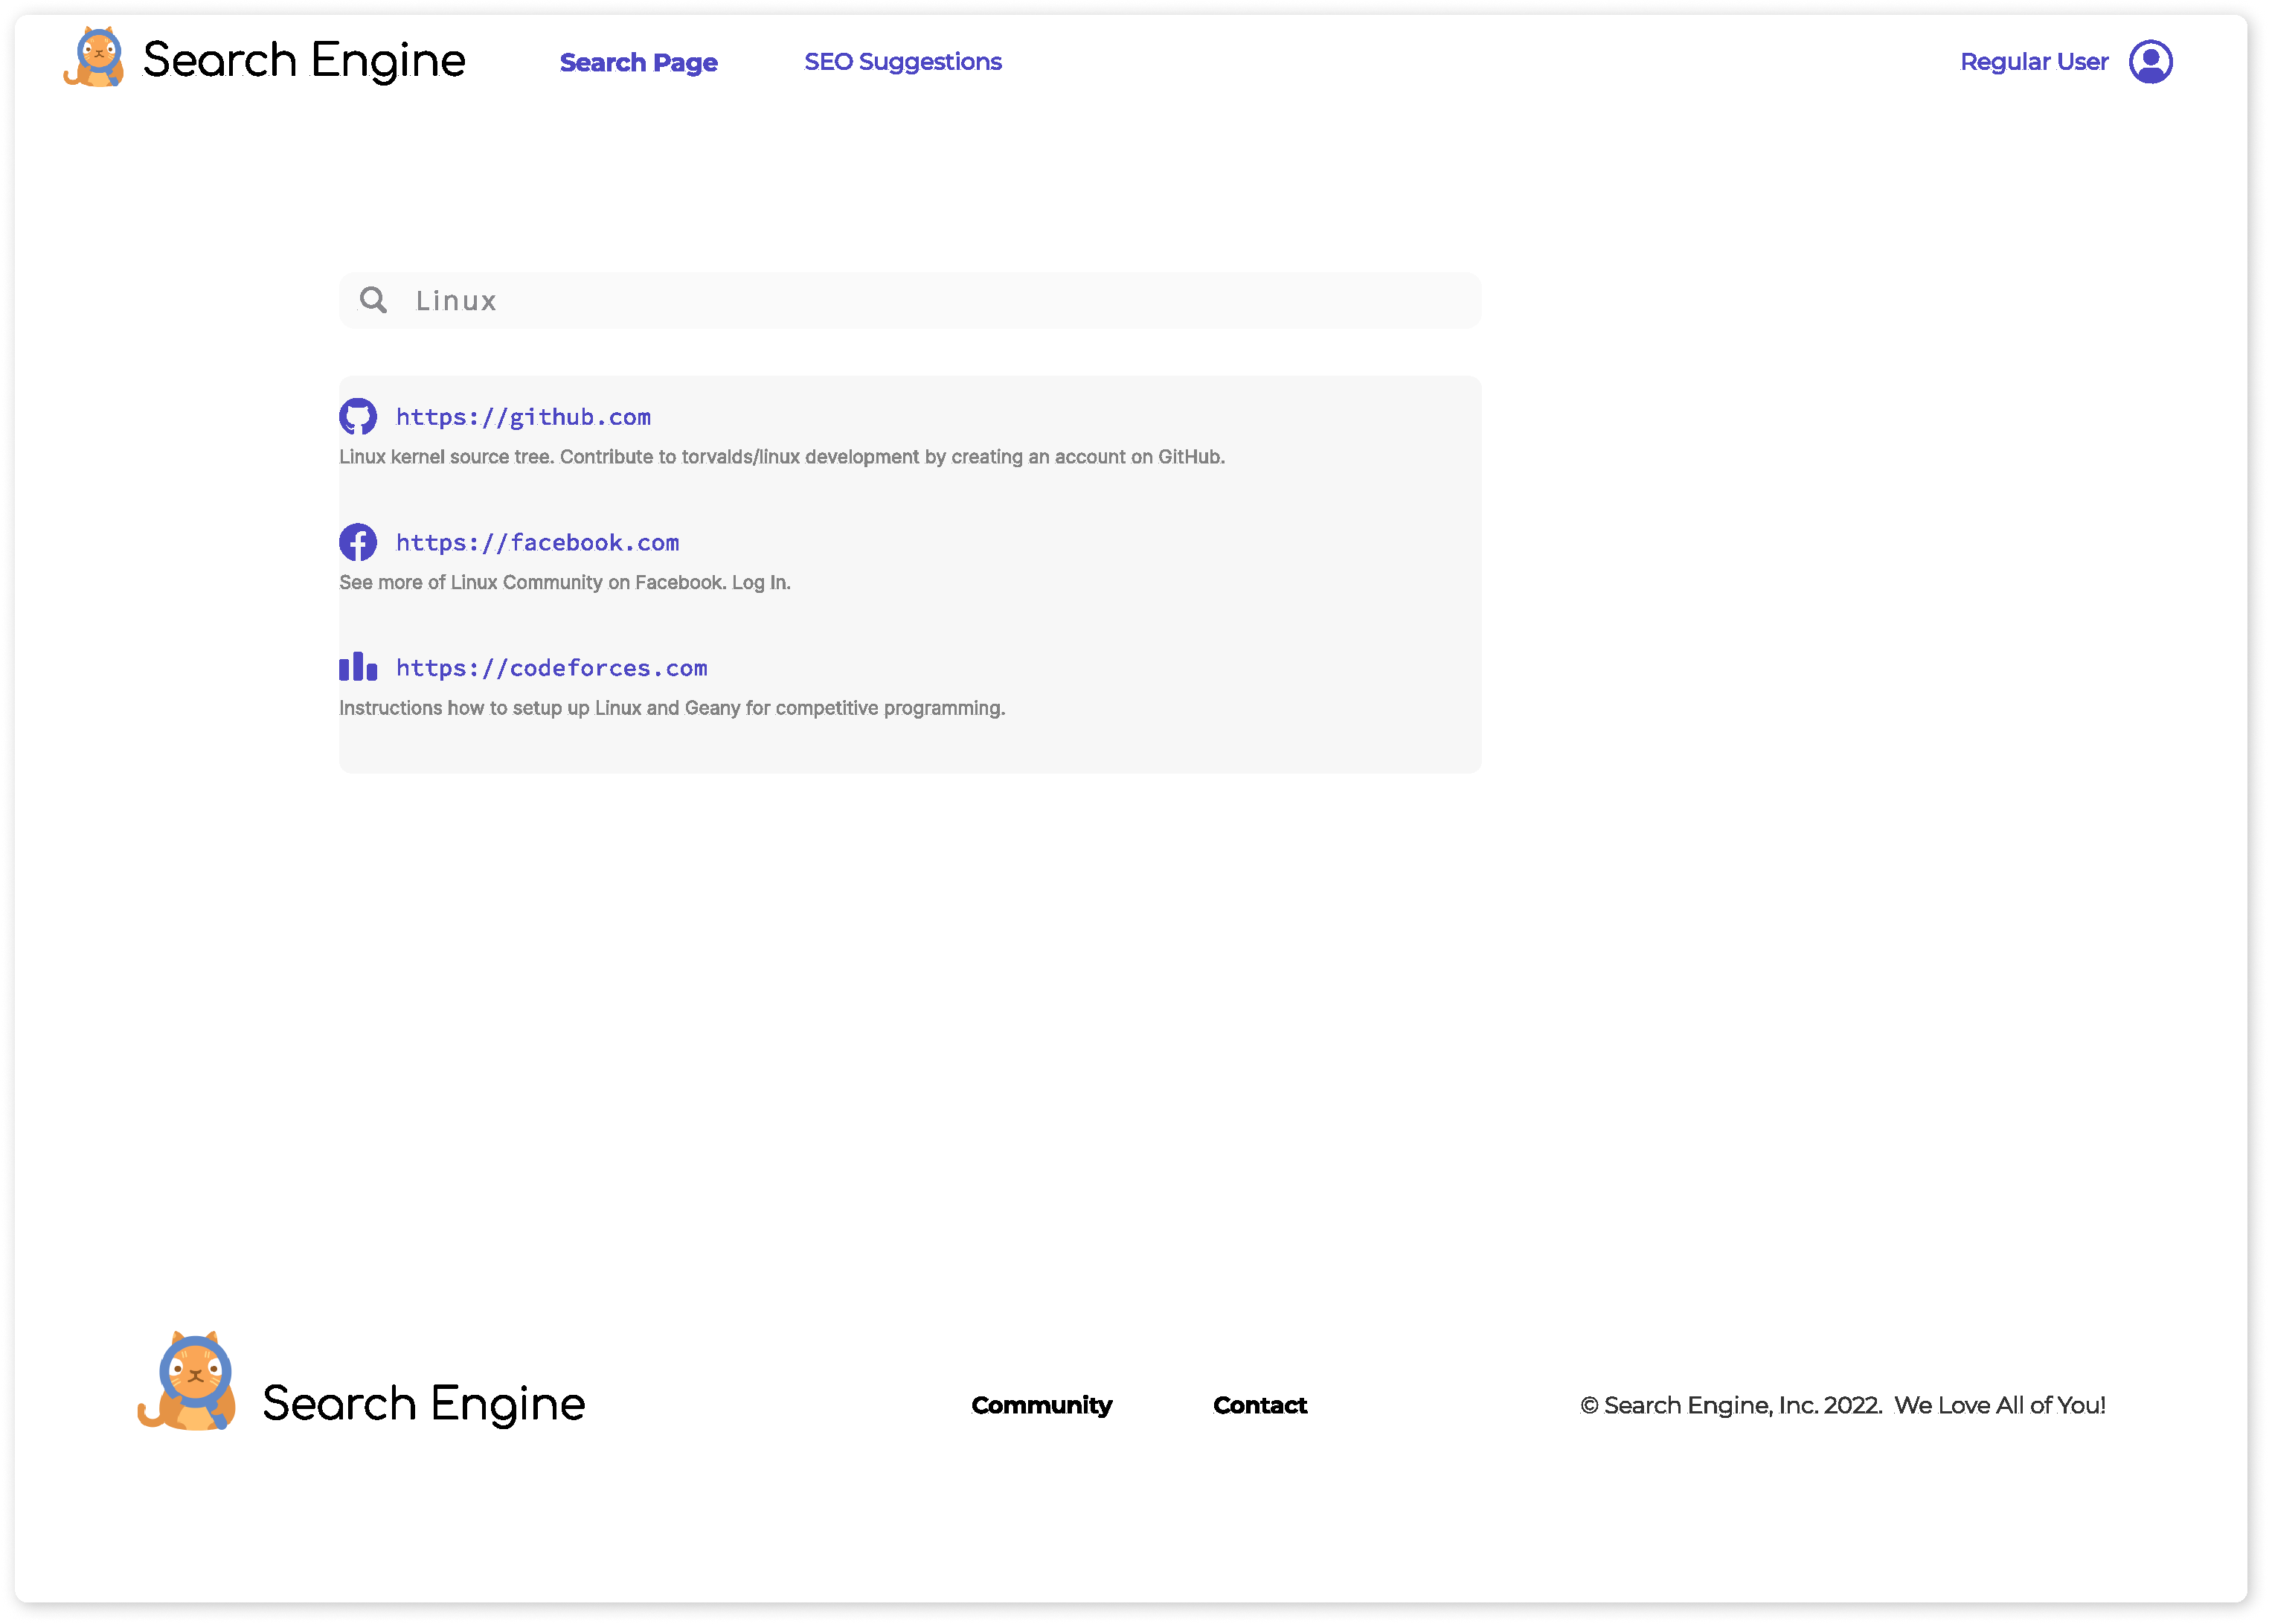
\includegraphics[width=0.90\textwidth]{search-result.pdf}
  \caption{Search Result}
\end{figure}

\begin{figure}[H]
  \centering
  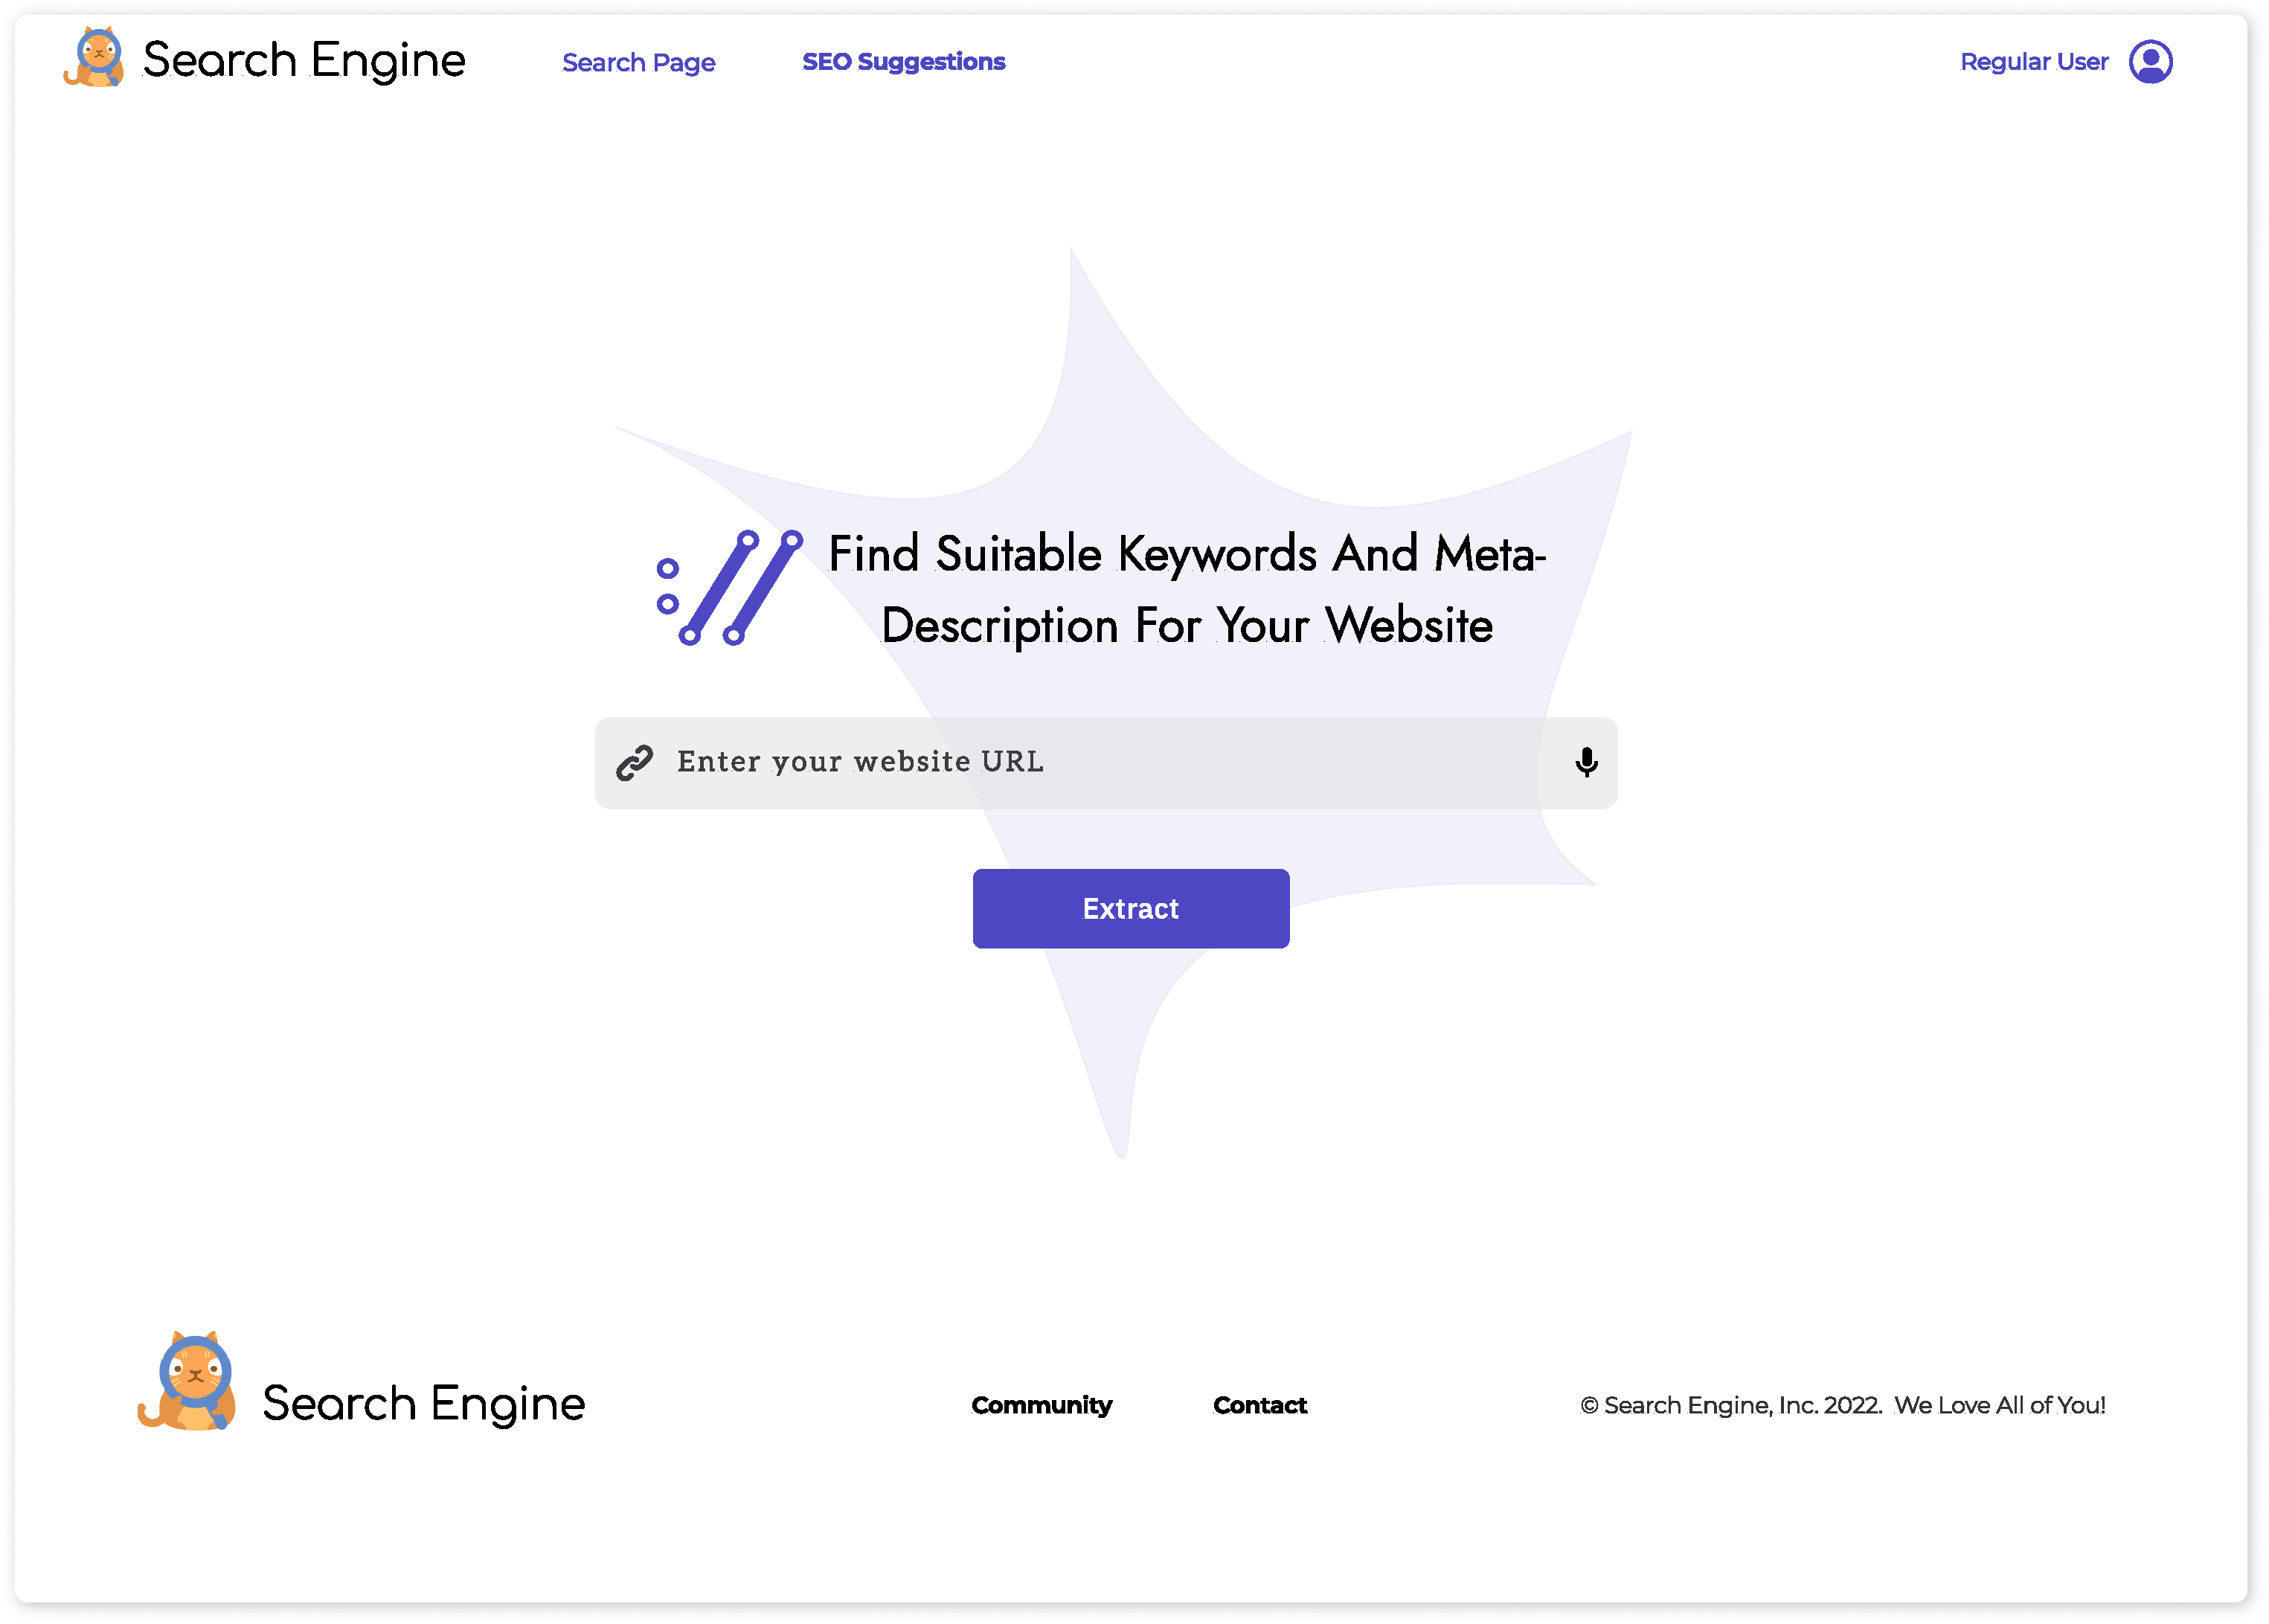
\includegraphics[width=0.90\textwidth]{seo-suggestions.pdf}
  \caption{SEO Suggestions Search}
\end{figure}

\begin{figure}[H]
  \centering
  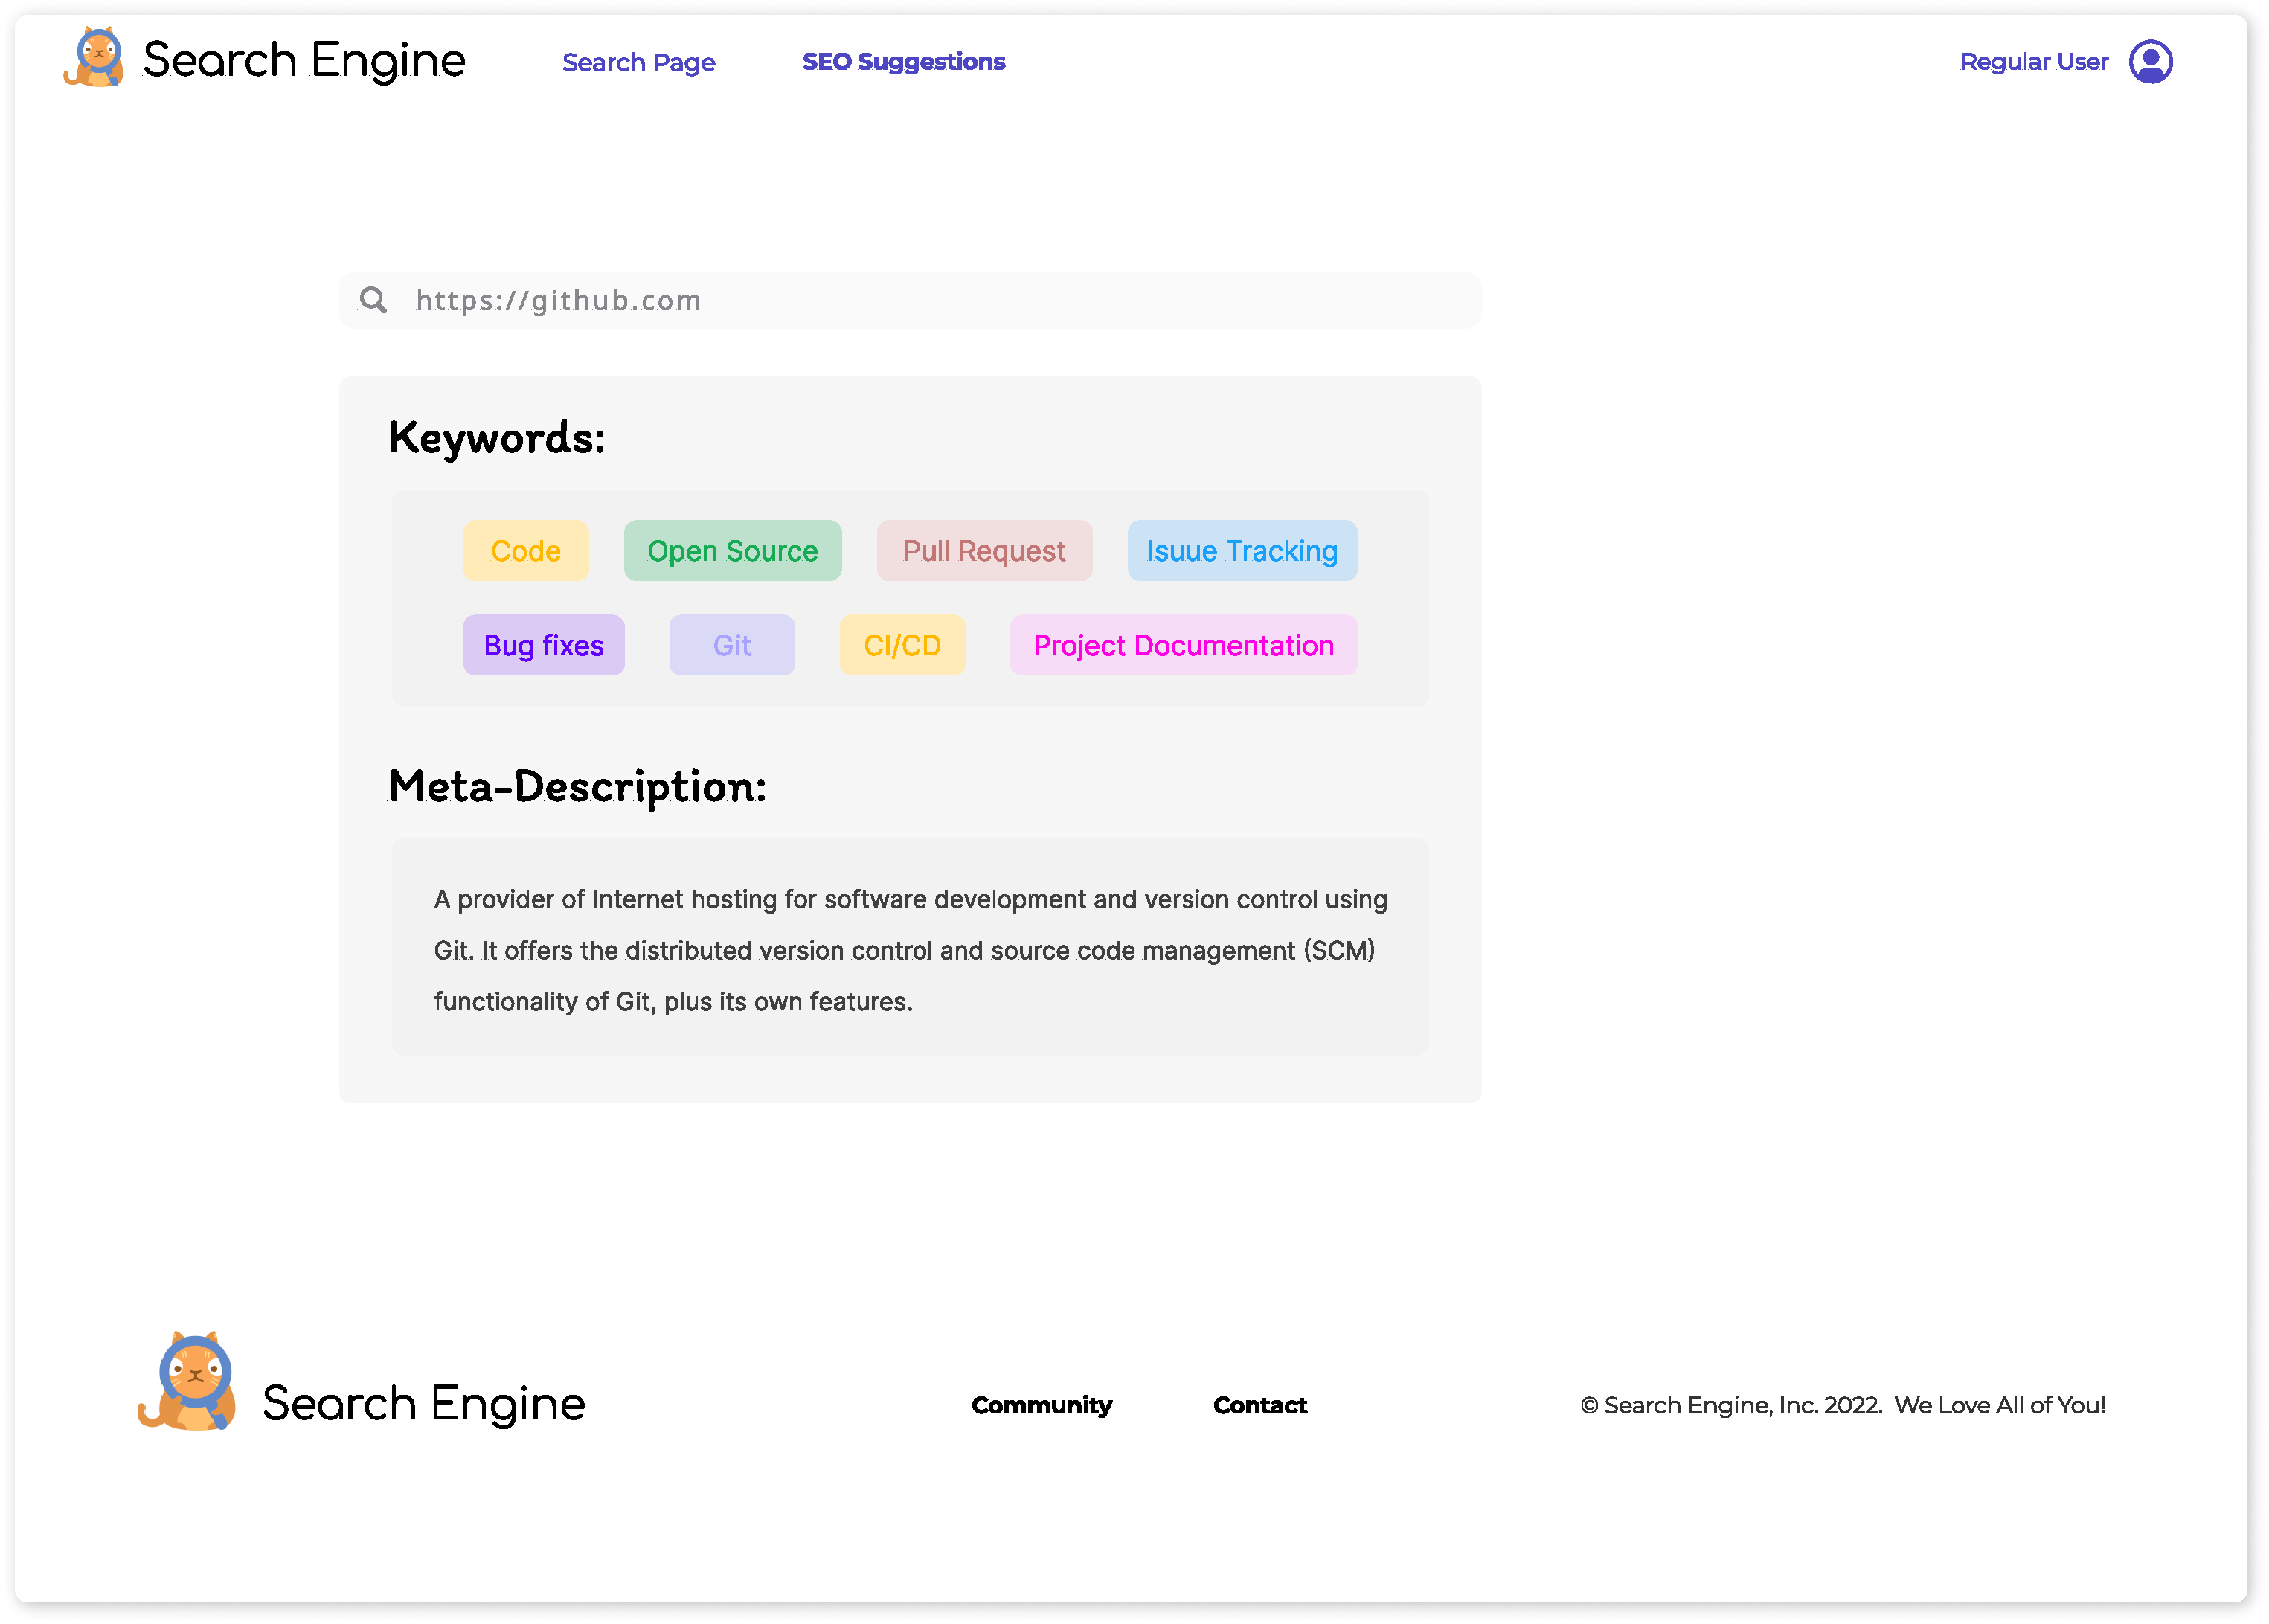
\includegraphics[width=0.90\textwidth]{seo-suggestions-result.pdf}
  \caption{SEO Suggestions Result}
\end{figure}

\end{document}